%!TEX root = main.tex
\vspace{-10pt}
\section{Perspective Resolution\label{perspective}}
% \subsection{Worker Clustering}
As discussed in Section~\ref{sec:error}, disagreements often arise in segmentation due to differing worker perspectives on large tile regions. We developed a clustering-based preprocessing approach to resolve this issue.
% is based on the intuition that workers with similar perspectives  will have segmentations that are closer to each other. 
Based on the intuition that workers with similar perspectives will have segmentations that are close to each other, we compute the Jaccard similarity between each pair of segmentations and perform spectral clustering to separate the segmentations into clusters. Figure \ref{error_examples} (bottom) illustrates how spectral clustering divides the worker segmentations into clusters with meaningful semantic associations, reflecting the diversity of perspectives for the same task. Clustering results can be used as a preprocessing step for any quality evaluation algorithm by keeping only the segmentations that belong to the largest cluster, which is typically free of semantic errors.
    \begin{figure}[h!]
      \centering
      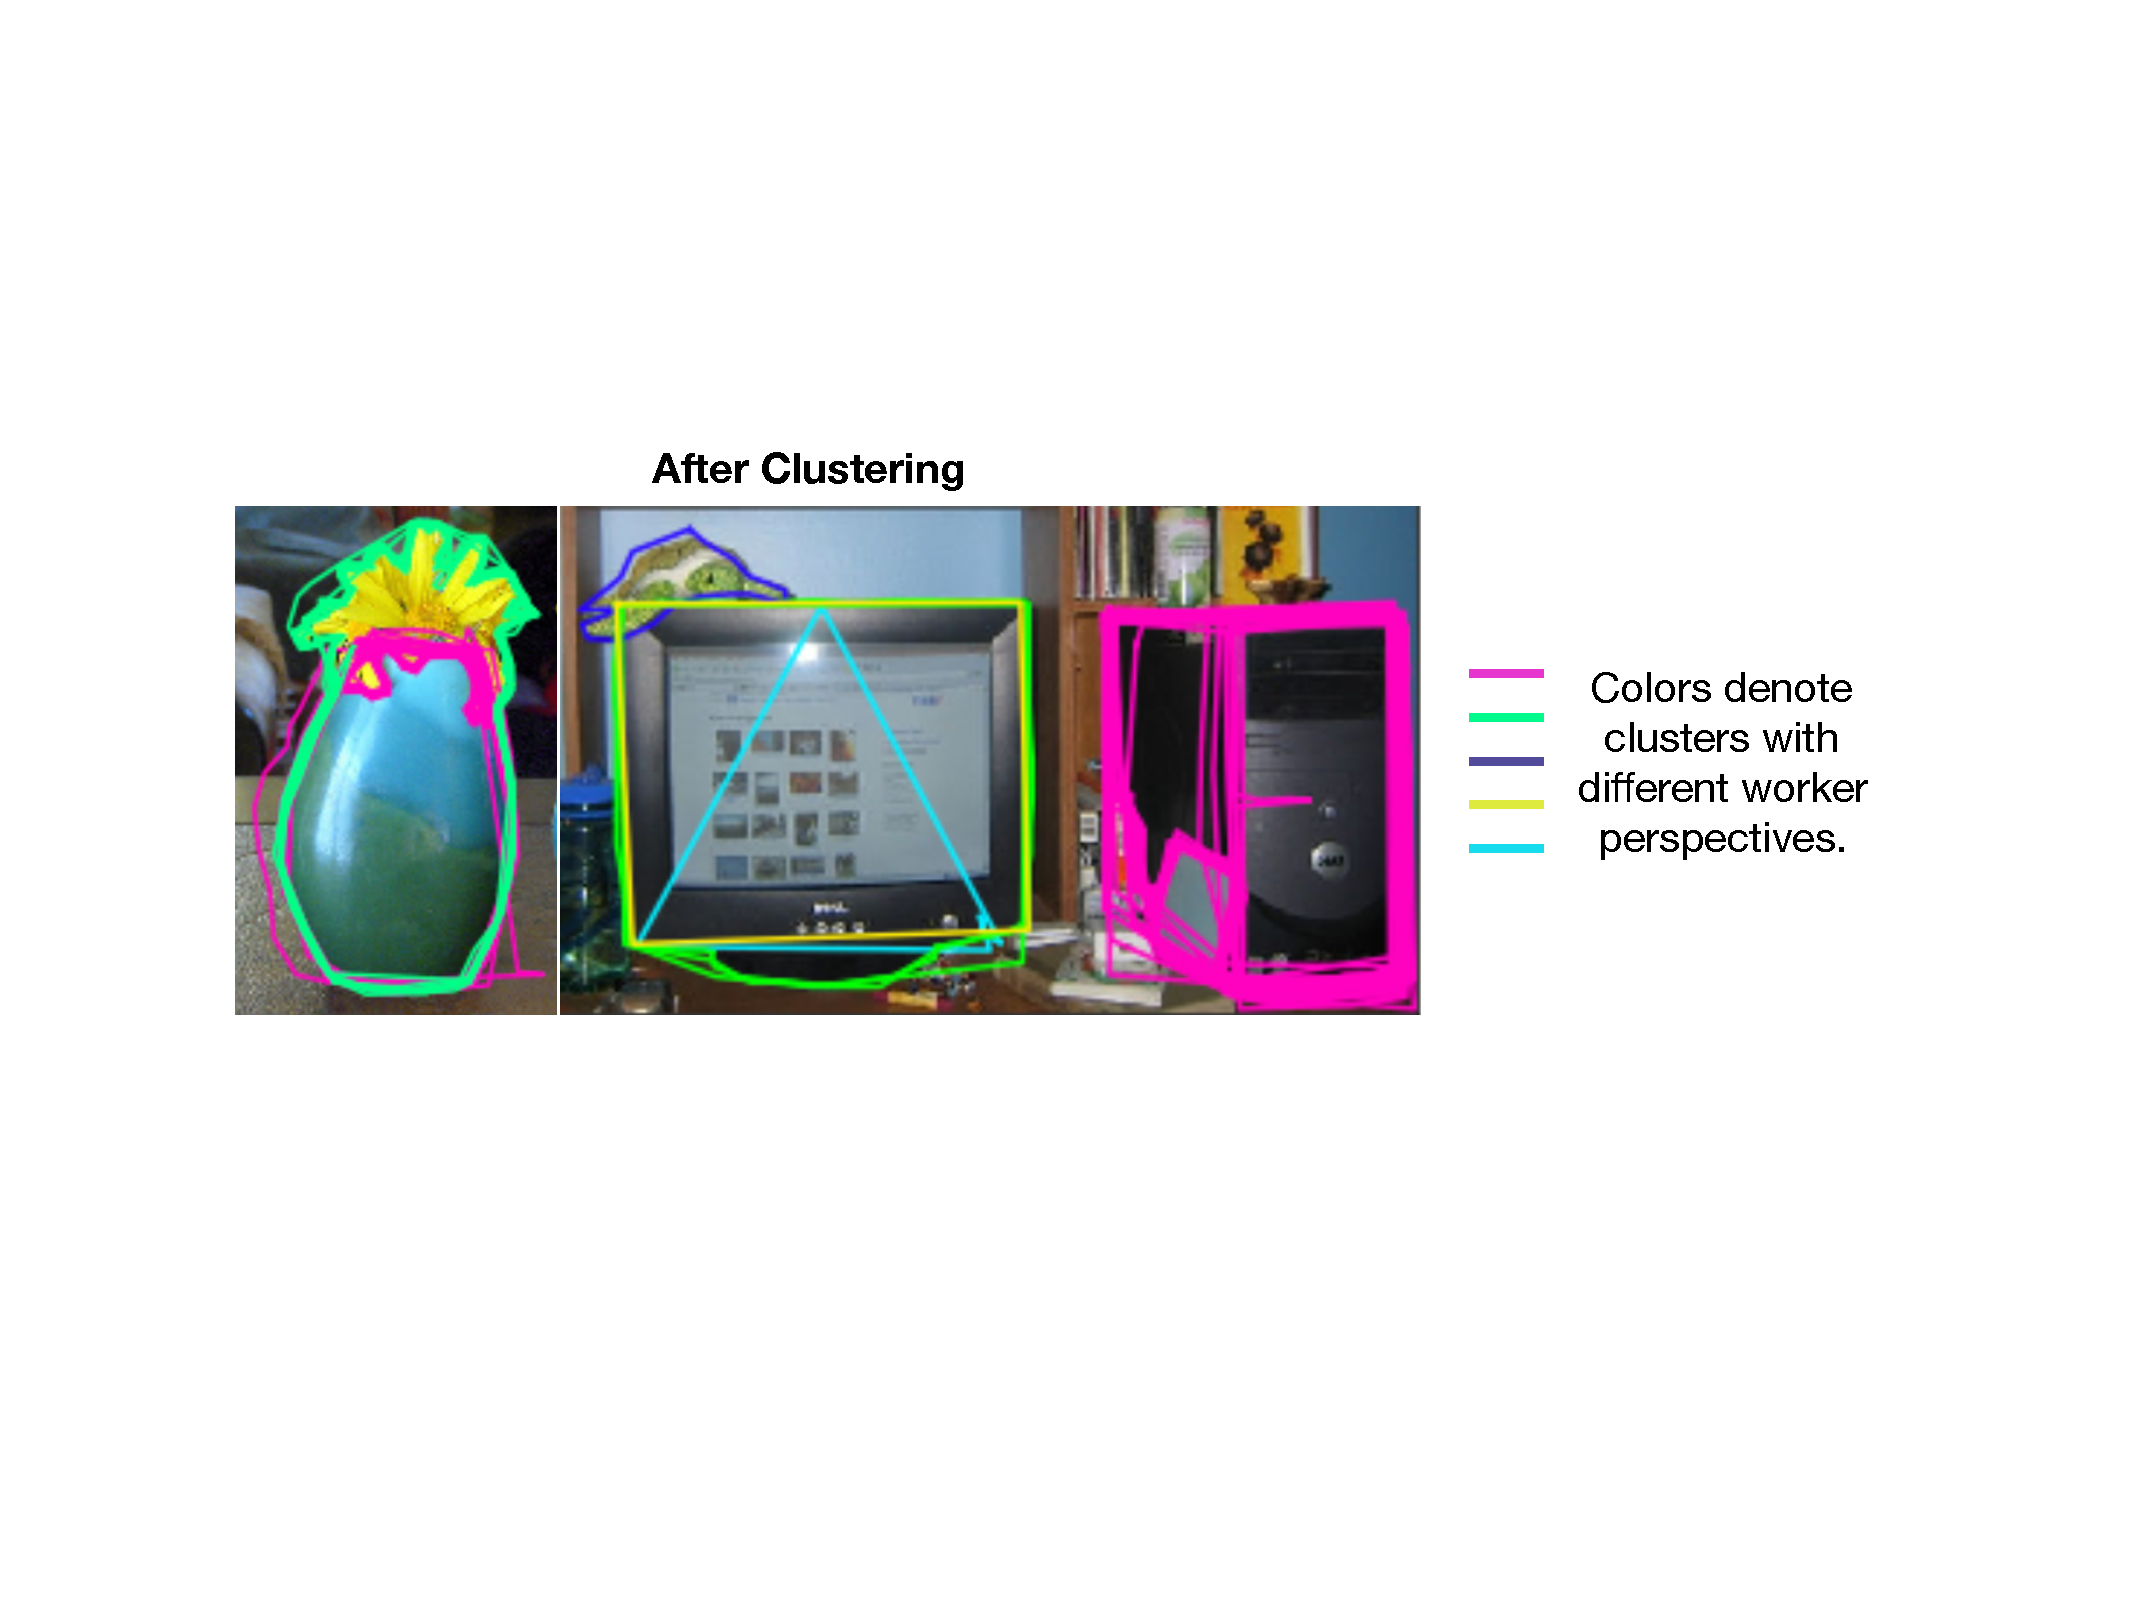
\includegraphics[width=\linewidth]{plots/clustering.pdf}
      \caption{Example image showing clustering performed on the same object from Figure \ref{error_examples} left and middle.}
      \label{cluster_example}
    \end{figure}
\par In addition, clustering offers the additional benefit of preserving worker's semantic intentions. For example, while the green cluster in Figure~\ref{error_examples} (bottom right) would be considered \textit{bad} segmentations for the particular task (`computer'), this cluster can provide more data for another segmentation task corresponding to `monitor'. A potential future work direction would be to crowdsource the semantic labels for the computed clusters to enable the reuse of segmentations across multiple objects to lower costs.%the cost of data collection. %(which is cheaper and more accurate than segmentation)
%A potential future work includes adding additional crowdsourcing tasks for semantic labeling of clusters (which is cheaper and more accurate than segmentation) to enable reuse of annotations across multiple objects and lower the cost of data collection. 